\chapter{Linguistic Model Applications: NLP Semantic Tasks} 
\label{chap:wsd}
\begin{abstractchap}
This chapter contains the experiments we performed as applications of the proposed model. We address the use of the heterogeneous contexts, the structure of the network and the sparsity of textual data.
First, we propose a method to solve word sense induction and disambiguation. This task is an elementary semantic NLP task useful to build larger systems. In the first section of this chapter, we leverage the network presented previously and propose an algorithm that takes into account the structure of our model. Based on the real-world property of the network, we induce senses by grouping words that share a similar sense. We then assign these senses to target words. We show that our method improves on similar network-based methods. Furthermore, we analyze how each type of context behave in terms of performance for each target word tested.

Secondly, in the second section of the chapter, we explore the use of well-known multi-modal fusion techniques to solve two prominent Natural Language Processing tasks. Specifically, we focus on solving Named Entity Recognition and Word Sense Induction and Disambiguation by applying feature-combination methods that have already shown their efficiency in the multi-media analysis domain. We present a series of experiments employing fusion techniques in order to combine textual linguistic features. Our results show that the combination of textual features indeed improves the performance compared to single feature and the trivial feature concatenation. 
%Furthermore, we perform an extensive analysis on the importance of each feature relevance with respect to the senses and classes discovered in WSI/WSD and NER, respectively.

\end{abstractchap}

\minitoc
\section{Leveraging the Network Structure}
\subsection{Introduction}
\label{chap5:intro}
In this chapter we employ the model introduced before to propose a solution to both Word Sense Disambiguation (WSD) and Induction  (WSI) tasks. The intuition of our method is not original, as we will see, but still we address concerns that are not very well studied, namely the use of heterogeneous context features to solve semantic tasks while reducing the number of parameters compared to similar approaches. Indeed, we also analyze the difference provided by different types of contexts. Our method is evaluated with two important datasets, that of Semeval 2007 and 2010.

We begin by giving a description and and recalling the art for both tasks. Specifically, we identify what type of language network is used and how.
%from a linguistic-network point of view.
We then present the characteristics of our proposed method. Finally we describe and discuss the obtained results.

%\subsection{Linguistic Networks in WSD and WSI}
%\subsection{Related Work}

Word sense disambiguation, or WSD, is the task of examining a word in different contexts (we refer to a word in a particular context as an instance)  and determining which is the sense being used in each one of the contexts analyzed. Usually a list of senses from where to chose the correct one is given as an input. When this list is not available, WSD then becomes a different, complementary task: word sense induction, or WSI. WSI also analyses  tokens of a target word context but before assigning a sense to each of its instances, it first generates a list of possible senses from where to select from. 

\paragraph{Word Sense Disambiguation}
%In the literature \cite{2007.Sinha.Mihalcea.Unsupervised,2007.Tsatsaronis.WSDwithSpreading,2007.Navigli.GraphConnectivity,2009.Agirre.PersonalizedPageRankWSD,2010.Klapaftis.WSD.WSD.HierarchicalGraphs,2010.Siberer.GraphCooccurrenceWSD,2014.Moro.Navigli.EntityLinking_WSD}, WSD 
%2004.Mihalcea.SemanticNetworkPageRank,  2008.Agirre.Multilingual
%is usually solved using semantic networks (SN). Specifically, Wordnet and to some extent BabelNet or Wikipedia (considering an article as a single concept).

Recall that the general process used to solve WSD follows a two-step algorithm. Given an input text with a words to disambiguate, and their corresponding context, WSD systems accomplish the following:
\begin{enumerate}
\item Link target words (usually nouns, without stop-words and functional words) with their corresponding  sense (or synset in the case of Wordnet-like dictionaries) and extract their vertices and edges into a new, smaller SN. 
\item Apply a node ranking technique, usually a random walk based method, and select, for each ambiguous word in the input text,  its top ranking synset node as the correct sense.
\end{enumerate}


The differences in the methods, in general boil down to three aspects. Firstly, the type of semantic relation implied by the edges of the network. Secondly, the function used to  assign a weight to each edge, as well as its meaning. On the other hand, a common characteristic of these approaches is that, as said before, they all rely on semantic networks and thus are constrained by the limitations of such resources, mainly their static content and human annotated nature. We find that the use of a lexical knowledge base, such as Wordnet, is pervasive in this task. Indeed, new resources, such as BabelNet, solves to some extent the fixed (no new senses are included automatically) nature of this type of resources by leveraging the ever-evolving knowledge of Wikipedia. 

\paragraph{Word Sense Induction}We believe that in order to solve WSD in a truly end-to-end unsupervised way, one would need to automatically find a list of senses for a word without the help of pre-built semantic networks. 
%In that sense, researchers generally use lexical co-occurrence networks, or LCNs, and thus leverage the distributional hypothesis, to automatically discover senses for a given target word. Therefore, WSI graph-based methods \cite{2004.Veronis,2007.Klapaftis.UOY,2010.Navigli.InducingWordSenses.Triangles,2008.Klapaftis.WSIUsingCollocations,2011.DiMarco.Navigli.ClusteringWebSearch,2011.Jurgens.WSICommunityDetection} are tightly related to LCNs.
Unsupervised WSI is performed as follows:

Given an input document with a set of target words, coupled with a set of contexts (a target word in a unique context is called an instance), the goal is to discover a list of senses for each target word and then assign each instance in the document with an automatically generated sense. The common four steps used are the following:

\begin{enumerate}
\item Build a LCN, assigning tokens as nodes and  establishing edges between them if they co-occur in a given context (usually if they both appear in the same sentence, paragraph or fixed window of words).
\item Determine the weights for each edge according to a frequency metric. 
\item Apply a graph clustering algorithm. Each cluster found will represent a sense of the polysemous target word.
\item Match target word instances with the clusters found (the senses) by using the word context. Specifically, assign a sense to each instance by looking at the tokens in the context. This step is actually the word sense disambiguation task. 
\end{enumerate}	

As with WSD, while  LCNs used are mostly the same among approaches, there are certain moving parts that make up the difference between WSI approaches. The most common differences that   arise are:

\begin{itemize}
\item The clustering algorithm to find senses in the LCN graph.
\item The technique used to match context words to clusters.
\item The weight used in the graph edges.
\end{itemize}


WSI, while being a more flexible approach (language and word-domain independent, does not require human-made knowledge bases), its results are tightly linked to the quality of the clustering algorithm used on the language network built. 
%

%\paragraph{State of the art discussion}\label{sec:survey_disc}


With respect to the networks' structure, we find that few approaches include syntactic attributes into their model. We believe that finding semantic similarities can be improved by adding syntactic information not only  while using dependency relations but also by leveraging the constituency tree of each word. Moreover, using syntactic data along with semantic and/or lexical co-occurrences takes us into the heterogeneous network domain which has not been addressed in most of the approaches covered.
Being able to design new similarity metrics that deal with different types of information opens new avenues of research in the semantic similarity domain. % Finally, concerning the algorithms employed, few approaches make direct use of the graph Laplacian representation. New similarities could be defined using the Laplacian as a starting point. 




\subsection{Proposed Method}
	
%The cited works use a LCN as described before while other works such as \cite{2014.Tao.Qian.LexicalChainHypergraphWSI} represent the co-occurrence by means of a hypergraph schema. In short, a hypergraph structure is a graph generalization where an edge (called hyperedge) can link multiple vertices per edge and thus it is able to provide a more complete description of the interactions between several nodes.


Formally, the objective of WSI/WSD is the following: given a document $d$ with a set $T$ of  target words $tw \in T$ and the set $C$ with contexts for each target word $ct_{tw}$. 
Specifically, each paragraph represents the context  of a target word. A target word in a specific context is also called an instance.
% $tw$. %Each word $tw$ features several $ct$.
The goal is first to solve the WSI task, that is, automatically determine a list of senses for a given $tw$, and then assign one meaning from this list to each of its instances, the WSD task.
%
%As described before, WSI  is usually solved following four steps: (1) creation of a linguistic network, (2) determine the level of similarity between nodes within the network, (3) cluster nodes together, thus creating individual senses, and (4)  assign a cluster (sense) to each instance of a target word in the input document (this step amounts to WSD).


Our method follows is inspired on previous approaches from \cite{2004.Veronis} and \cite{2007.Klapaftis.UOY}. In Hyperlex,  the graph-based  method presented  in \cite{2004.Veronis}, the main intuition is that co-occurrence networks have small-world properties and thus it is possible to detect and isolate important heavily-connected nodes, call "hubs". These hubs, and their connected nodes represent a sense in itself. 

Hyperlex performs WSI and WSD using a weighted lexical co-occurrence network. The process is performed for each target word in the document. As a first step, they build a  graph by defining the vertices (the target word node is removed) as the tokens found in the  co-occurring  context of a target word. The edges link two words co-occurring together. Each edge is assigned a weight that decreases as the association frequency of the words increases. The second step consists on iteratively finding the hubs and removing them, along with their adjacent nodes, from the target word graph. Again, the intuition of the method is that these isolated hubs, and their adjacent words, represent a sense of the analyzed word. The third and final step carries out the disambiguation. A new graph is created by adding the target word to the co-occurrence graph. Zero-weighted edges are added between each hub and the target word. A minimum spanning tree is then calculated and the sense component found to have the closest set of nodes is chosen as the target word sense.

The second approach, \textit{UOY}, described in \cite{2007.Klapaftis.UOY},  relies itself on the small-world intuition presented  by Hyperlex to find hubs and its adjacent nodes to represent senses.   In short, these methods, as ours, exploit the real-world characteristics of linguistic networks by theorizing that there are certain few high-degree nodes (called hubs) that carry an important role in the network and therefore may represent, coupled with their neighbors, a sense for a given target word. Particularly, UOY considers bigrams and trigrams that co-occur in a paragraph as hyperedges. Under a frequent-itemset setting, they determine important hyperedges given their \textit{support} and their \textit{confidence}  values. Then, the clustering of words takes place by finding the hubs and considering them as sense carriers only if they satisfy a threshold mainly set upon their containing-hyperedge confidence value. Finally, once the senses are identified, each target word instance (represented by a context) is assigned to a sense according to the sum of confidences of the hyperedge appearing on said context. 

In our method, we generate a network for each $tw$ and consider that the high-degree nodes inside this network may represent a $tw$ sense. Figure \ref{fig:wsd_wsi_process}  shows an overview of the process. Also, in Algorithm \ref{alg:wsd} we show the general flow of our approach.  We detail the steps taken alongside the corresponding line in the algorithm below. 

\begin{figure}
\centering
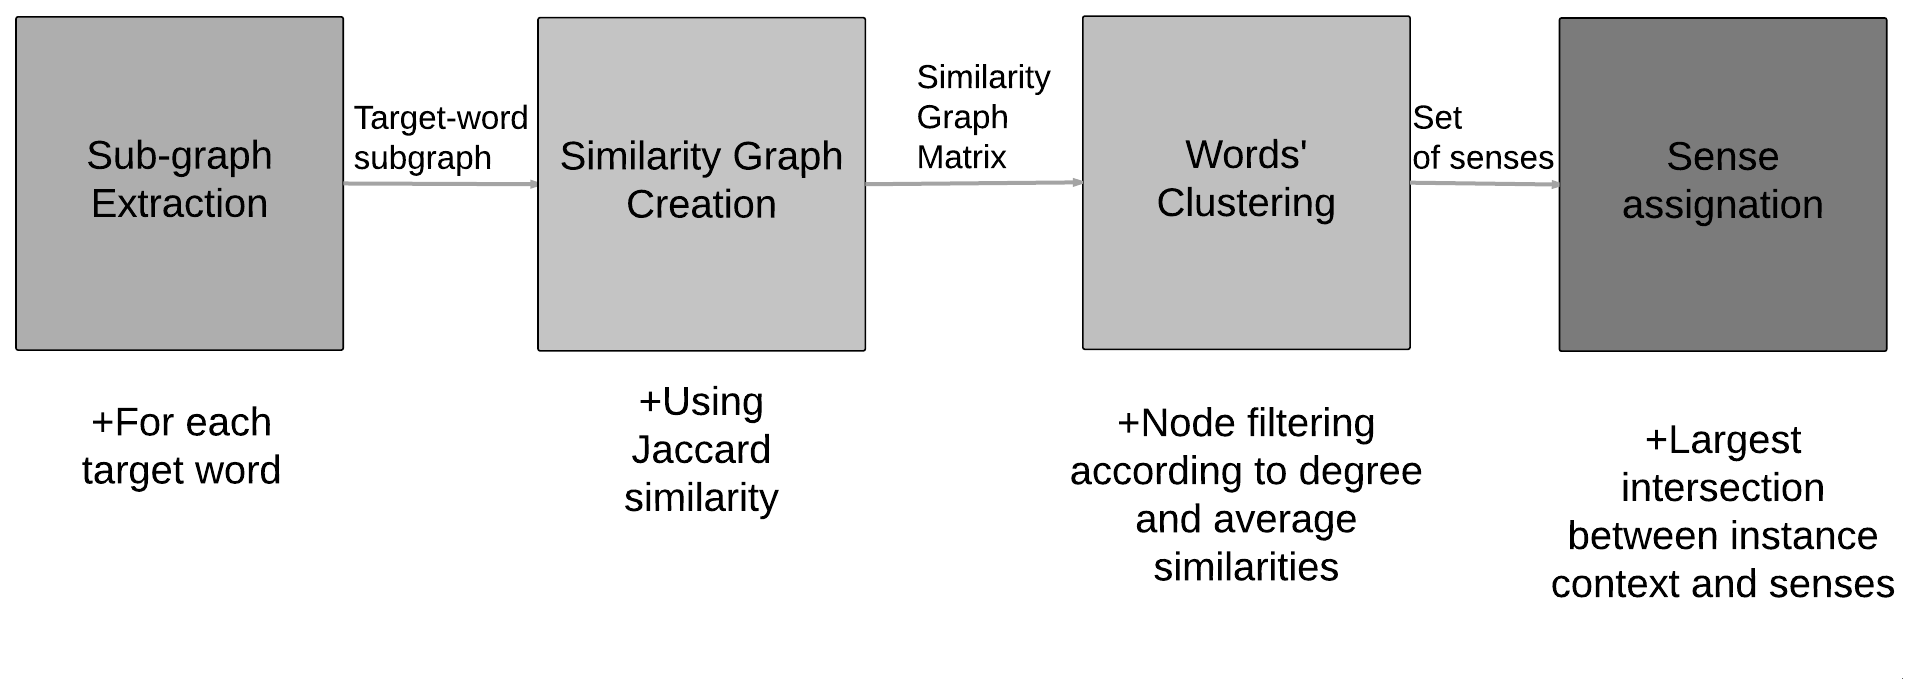
\includegraphics[width=1\linewidth]{images/Chapitre4/wsd_wsi_process.png}
\caption{Block diagram of the WSI/WSD method proposed.}
\label{fig:wsd_wsi_process}
\end{figure}


\paragraph{Creation of the linguistic network}
%In the previous sections we worked with the English Wikipedia as background corpus to build and model our proposed linguistic network. Given the large size of Wikipedia, and to iterate faster our experiments, we decided to change the corpus to one with a more manageable size.

%We use the Open American National Corpus (OANC) \cite{oanc} as background document collection to build a hypergraph network $G_H$ following our proposed model.  The OANC  includes texts from several domains and encompasses 11,406,155 words. We split the documents of the corpus in sentences, then we tokenize and parse them with Stanford's CoreNLP \cite{corenlp}. As described before, the dependency and constituency tree are used to build the hypergraph: words are depicted by nodes, and they may exist inside any of the three different types of hyperedges defined (sentence,  noun phrase or dependency contexts). If any  hyperedge is repeated through the corpus, we increment a counter and keep the number of apparitions instead of adding redundant columns to the hypergraph incidence matrix.

In order to find senses from the contexts of a target word, the first step in our procedure is to build a linguistic graph $G_H$ from a background corpus. As described in previous sections, the dependency and constituency trees are used to build the hypergraph: words are depicted by nodes, and they may exist inside any of the three different types of hyperedges defined (sentence,  noun phrase or dependency contexts). If any  hyperedge is repeated through the corpus, we increment a counter and keep the number of apparitions instead of adding redundant columns to the hypergraph incidence matrix.

At each step, that is, for each $tw$ in the test input document, we extract a subgraph $G_{tw}$ from $G_H$ that contains all the words that appear together with $tw$ (line 2), whether by lexical or syntactic co-occurrence. The $tw$ is removed from $G_{tw}$. In this approach we focus specifically on dependency relations and lexical co-occurrence. 

We note that for the syntactic co-occurrence, that is, the dependency relations between words, we apply two strategies: when dealing with a noun target word, we use the co-occurrent relations between said noun and other words having a similar head dependency token. On the other hand, when dealing with verbs, we select the co-occurrent words having said verb as head of the dependency relation.  

\paragraph{Computing the similarity between nodes}
In order to computationally treat $G_{tw}$, we first induce a bipartite graph $B_{tw}=(U,W,E)$ from $G_{tw}$ (line 3). The set of left nodes $U$ represent words and the set of right nodes $W$ depicts the membership to a given hyperedge. Thus, we have as many nodes in $W$  as we had hyperedges in $G_H$.

We compute the Jaccard index between each node $n_{i,j} \in U$ as $Jaccard(i,j)=\frac{|N(i)\cap N(j)|}{|N(i)\cup N(j)|}$ in order to build a $|U|\times|U|$ similarity matrix $S_{tw}$ (line 4). We induce from $S_{tw}$ a new filtered  hypergraph incidence matrix $F_{tw}$ (line 5), which contains word nodes as rows and columns as hyperedges. Each of these hyperedges represent a set of words that are deemed similar between them according to their Jaccard  index value, which must be equal or higher than an assigned threshold $th_1$ .  

\paragraph{Clustering words  together}
Once the incidence matrix $F_{tw}$ is built we can proceed to induce senses for a target word by clustering words (vertices) together. First, we calculate the degree of each node $n_i \in F_{tw}$. The degree of a node is simply the number of hyperedges it is incident in. Nodes are sorted in descending order and evaluated one by one. We consider the top $c$-nodes as sense hub candidates (line 6). We accept or reject a node $n \in F_{tw}$ as a sense carrying word according to one condition. As shown from line 11 to 17 in the pseudo-code, we set a minimum limit to the average of the Jaccard similarities between each pair of neighbors of node $n \in F_{tw}$ within each hyperedge  $n$ belongs to. Formally, for a node $n$, we define the average Jaccard measure as: $$AvgJaccard(n)=\frac{1}{|hedges(n)|}\sum_{h\in hedges(n)}\frac{\sum_{\substack{i\in h\\j\in h;i\neq j}}Jaccard(i,j)}{|h| + 1}$$ 
where $hedeges(n)$ is the set of hyperedges $n$ is incident in and its cardinality is defined as $|hedges(n)|$. $|h|$ is the number of nodes in hyperedge $h$. 

The Jaccard similarity measure allows us to easily determine the neighbors of each node in the current bipartite hypergraph representation. As each node is joined to a sentence or dependency node, calculating the Jaccard similarity amounts to determining the level of co-occurrence between each word according to a specific type of hyperedge (represented as a node from the other graph partition) while taking into account the total number of hyperedges the words participate in. We differentiate specifically from the previously described method, UOY, in that in the case of that system, the weighting of the hyperedges is done by computing the average confidence metric of each hyperedge. In this regard, the Jaccard similarity is more flexible with respect to the confidence metric, as the confidence requires in the numerator the number of contexts (paragraphs in UOY's case) shared by all the members of the hyperedge, whereas the Jaccard measure takes pairs of members individually and thus is less strict in the apparition of all the elements of the hyperedge in the contexts. Given the nature of the features used (lexical and syntactical dependencies), we fix our thresholds in a manual but simpler way by defining percentiles and taking the value of the threshold directly, without having to change it according to the characteristics of the data.

If node $n$ satisfies both thresholds $th_1$ and $th_2$, it is deemed as a sense purveyor and all its neighbors (words that appear in the same hyperedges as $n$) are conflated into a single set representing a $tw$ sense. This new sense is added to $SoS_{tw}$ (line 17). The sense set is then removed from $F_{tw}$.

The process is repeated until no more nodes satisfy both boundaries. When the process is complete, we obtain a set of senses $SoS_{tw}$ where each set contains words that ideally represent a unique meaning for each target word. 

\paragraph{Sense assignation}

The assignation of a sense consists in looking at each $tw$ instance represented by a context $ct$ and simply determining which sense $s$ in $SoS_{tw}$ shares the highest amount of words with $ct$. The sense $s$ is thus assigned to that instance. If two senses in $SoS_{tw}$ share the same amount of words with $ct$, one of them is randomly chosen.  This operation is repeated for each instance of each target word. 


~

\begin{algorithm}[]
\SetAlgoLined
\KwIn{A set $tw\_set=\{tw_1, tw_2, ..., tw_n\}$ of target words }
\KwIn{A background linguistic network $G_H$}
\KwIn{Filtering thresholds $th_1$, $th_2$}

\KwOut{A set $SoS_{tw}$ of senses for each target word}
\ForEach{target word $tw$ in tw\_set}{
	
	$G_{tw}$ = \texttt{extract\_subgraph}($G_H$, $tw$)\;
	$B_{tw}$ = \texttt{induce\_bipartite\_graph}($G_{tw}$)\;
	$S_{tw}$ = \texttt{sim\_matrix}($B_{tw}$)\;
	$F_{tw}$ = \texttt{induce\_hypergraph}($S_{tw}$, \textit{th1})\;
	$candidate\_hubs$ = \texttt{sort(degree}($F_{tw}$))[:100]\;
	$SoS_{tw}$ = [~]\;
	\ForEach{candidate\_hub in candidate\_hubs}{
%		\uIf{\texttt{degree}(candidate\_hub) $<$ th2}{
%			\textbf{continue}\;
%			}
%		\tcc{get all hyperedges where candidate\_hub appears}
		$candidate\_hyperedges$ = \texttt{get\_hyperedges}($candidate\_hub$, $F_{tw}$)\;
		$candidate\_avg_jaccard$ = 0\;
		\ForEach{ hyperedge in candidate\_hyperedges}{
%		\tcc{get average jaccard of all words (nodes) within hyperedge}
			$candidate\_avg\_jaccard$ += \texttt{get\_avg\_jaccard}($hyperedge$)\;
			}
		\uIf{candidate\_jaccard $>$ th2}{
			$SoS_{tw}$.\texttt{add}(\texttt{get\_words}($candidate\_hyperedges$))\;
%			\tcc{remove hyperedges of candidate hub from tw (filtered) hypergraph.}
			$F_{tw}$ = $F_{tw} \setminus candidate\_hyperedges$\;
		}
	}
	\Return{$SoS_{tw}$}
}

\caption{Pseudo-code of our WSI/WSD network-based approach}
\label{alg:wsd}
\end{algorithm}

	
\subsection{Experiments and Evaluation}

\subsubsection{Datasets}
We trained and evaluated our system on two datasets: Semeval-2007 (task 2) \cite{semeval2007task2} and Semeval-2010 (Task 14) \cite{Semeval2010}. The Semeval-2007 task consisted in the induction and disambiguation of a single set of 100 words, 65 verbs and 35 nouns, each target word having a set of contexts where the word appear. On the other hand, the Semeval-2010 task consisted also on 100 words, with 50 being verbs and 50 being nouns. This time, a training set from which the senses of a word have to be induced is provided. In our experiment, for the Semeval-2010 dataset, we induce the senses from the training set and disambiguate the target words within the test set.

We apply a light pre-treatment, consisting on token lemmatization and we remove all words that appear less than four times. Concerning the individual graphs of each target word, we work only with nouns and if the extracted graph has fewer than 100 nodes, we do not apply any filtering (we keep all the extracted words). We do this in order to avoid empty solutions.



\subsubsection{Implementation}
The objective of this experiment is to show the complementarity of both lexical and syntactic co-occurrence information while solving WSI and WSD tasks while using the method described in the previous subsection. To that end we build two independent systems: \textbf{LEX}, which uses exclusively lexical co-occurrence hyperedges, and \textbf{DEP}, which employs only syntactic dependency hyperedges. 
 %
Each type of hyperedge has its own network characteristics as mentioned before. Sentence hyperedges tend to have a much smaller number of words than those of the dependency category. This make sense as sentences usually contain less than 30 words, meanwhile a dependency hyperedge may contain up to hundreds of words (several words may share the same dependency relation). Taking this into consideration we set different threshold values for \textbf{LEX} and for \textbf{DEP}. First, we  consider only the top 100 nodes as candidate sense hubs. Secondly, we do not set the thresholds' values directly but instead we set up a percentile value for the Jaccard similarity ($th_1$) and for the average Jaccard similarity ($th_2$). This is a practical solution to the changing nature of the network model according to the features being employed. We experimentally found the best values for  each threshold used.



%Given that the variation of these thresholds affect the performance of the systems, we decided to experimentally fix threshold $th_1$ at 0.7 for \textit{dep} and at 0.030 for \textit{lex}. The difference of scales is determined by the characteristics stated before, that is, the sparse nature of the sentence hyperedges compared to the density of dependency hyperedges. The second threshold $th_2$ is automatically set for both systems, as explained above.
%
%This leaves only one threshold left, $th_3$. We experiment with two different ranges of values, one for each system. For \textit{dep} we set the range $[0.3, 0.65]$ with a step of 0.05. For \textit{lex} we set $[0.01, 0.08]$ with a step of 0.1. These ranges were chosen experimentally with two constraints in mind: (1) lower threshold values usually gave the same results\footnote{Still, some of the values used produced equal results and thus are not visible in Figure \ref{fig:prec_recall}.} as those already included in our ranges, and (2) higher threshold values forced the system to either give only one sense per word (resulting in the most frequent baseline), or even worse, not accepting any sense, thus having an null solution. 



\subsection{Results and Discussion}
Both Semeval-2007 and Semeval-2010 tasks are evaluated by an unsupervised and supervised set of measures. 
\paragraph{Semeval-2007}
In the case of Semeval-2007, the unsupervised evaluation assumed the induced senses as clusters of examples. These clusters are compared to the sets of examples tagged with the given gold standard word senses (classes), and evaluated using the \textit{F-Score} measure for clusters. 
 
The supervised setting maps the induced senses to manually-defined gold standard senses, and use a mapping produced by the organizers to tag the test corpus with gold standard tags. The mapping is
automatically produced by the organizers, and the resulting results evaluated according to the
usual precision and recall measures for supervised word sense disambiguation systems. 


In Table \ref{tab:sem2007_unsup_FS} we present the unsupervised evaluation results for our models as well as for some other systems. We include the F-Score measure as performance metric. Three baselines are included. The best one, one cluster per word, or \textit{1c1word} was not beaten during the competition. The second was a random assignation of senses to each instance. Finally, the third and easiest to beat baseline assigned one cluster per instance {1c1instance}. 

In this table, as in the rest of the tables presented in this section, the columns show the results for all the words, for the nouns exclusively as well as for the verbs. The final column indicates the number of induced clusters per system. It is important to consider this value as the unsupervised metrics are biased towards systems with less number of induced clusters and thus to the 1c1word baseline.

We can appreciate that both our methods surpass the baselines and the system described before \textit{UoY(2007)}. The best system of the competition, \textit{UBC-AS} used also co-occurrence graphs and applied a random-walk based clustering algorithm over the vertices' similarity matrix. Still, our system induced a larger amount of senses, while retaining a competitive F-Score value. We also note that in this evaluation \textbf{DEP}, the system using only co-occurrent dependency relations outperformed the lexical co-occurrence only system \textbf{LEX}.

Moving onto the supervised results for Semeval-2007, in Table \ref{tab:sem2007_sup_recall} we show the results obtained concerning the Recall performance metric.  In this table we include the competing system \textit{I2R}, based on an Information Bottleneck based clustering algorithm, which obtains the best results according to all the words and nouns. Both our systems \textbf{DEP} and \textbf{LEX} beat the baseline of assigning the most frequent sense to an instance (\textit{MFS}). More interestingly, \textit{DEP} was able to beat the MFS verb baseline, something that was not achieved during the competition. As was the case before, our systems beat UoY(2007).




As a way of determining where does both systems complement each other, in Figure \ref{fig:nouns_fs} and Figures  \ref{fig:verbs_fs2} and \ref{fig:verbs_fs3} we show the unsupervised F-Score value for nouns and verbs respectively (we split the verbs in two figures for visibility). We can see that, as the previous result tables indicated, \textbf{DEP} did better overall. Nonetheless, and what is most interesting in these figures, is that there are certain words, nouns and verbs, that obtain better scores using \textbf{LEX} instead of \textbf{DEP} and vice versa. For example, the nouns \textit{area}, \textit{future}, and \textit{state} are better treated by \textbf{SEN}, according to this measure, even if by a small margin. On the other hand, with respect to the verbs, the differences between performance are more important. The system \textbf{SEN} does better while finding senses and assigning them to the verbs \textit{avoid}, \textit{fix}, and \textit{work}. This information will be useful during the design of hybridization techniques between feature of our hypergraph structure.

 

% Please add the following required packages to your document preamble:
% \usepackage{booktabs}
\begin{table}[!htb]
\centering

\begin{tabular}{@{}lrrrr@{}}
\toprule
\textbf{FS (\%)} & \textbf{all} & \textbf{nouns} & \textbf{verbs} & \textbf{\#cl} \\ \midrule
1c1word          & 78.9         & 80.7           & 76.8           & 1.00             \\
UBC-AS           & 78.7         & 80.8           & 76.3           & 1.32          \\
\textbf{DEP}     & 74.9         & 80.2           & 69.0           & 3.27          \\
\textbf{LEX}     & 61.4         & 62.6           & 60.1           & 4.26         \\
UoY(2007)        & 56.1         & 65.8           & 45.1           & 9.28          \\
Random           & 37.9         & 38.1           & 37.7           & 19.7             \\
1c1instance & 	9.5         & 6.6           & 12.7           & 48.51             \\ \bottomrule
\end{tabular}
\caption{Unsupervised F-Score (FS) for the Semeval 2007 test set}
\label{tab:sem2007_unsup_FS}
\end{table}
 

% Please add the following required packages to your document preamble:
% \usepackage{booktabs}
\begin{table}[!htb]
\centering

\begin{tabular}{@{}lrrrr@{}}
\toprule
\textbf{SR (\%)} & \textbf{all} & \textbf{nouns} & \textbf{verbs} & \textbf{\#cl} \\ \midrule
I2R & 81.6 & 86.8 & 75.7 & 3.08 \\
\textbf{LEX} & 79.4 & 82.5 & 75.9 & 4.26 \\
\textbf{DEP} & 79.1 & 81.5 & 76.4 & 3.27\\
MFS & 78.7 & 80.9 & 76.2 & 1 \\
UoY(2007) & 77.7 & 81.6 & 73.3 & 9.28 \\ \bottomrule
\end{tabular}
\caption{Supervised Recall (SR) on the Semeval 2007 test set}
\label{tab:sem2007_sup_recall}
\end{table}



 \begin{figure}[!htb]
\centering
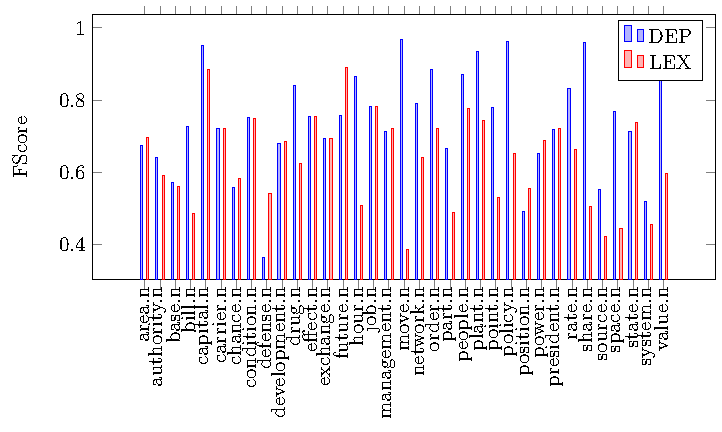
\includegraphics[width=1\linewidth]{images/Chapitre5/tex_img_files/nouns_fs.pdf}
\caption{Unsupervised F-Score results for the nouns of the Semeval 2007 test set.}
\label{fig:nouns_fs}
\end{figure}

 \begin{figure}[!htb]
\centering
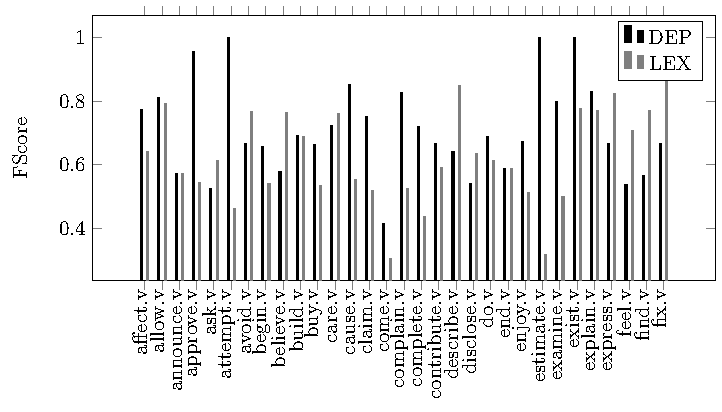
\includegraphics[width=1\linewidth]{images/Chapitre5/tex_img_files/verbs_fs_2.pdf}
\caption{Unsupervised F-Score results for the first half of verbs of the Semeval 2007 test set.}
\label{fig:verbs_fs2}
\end{figure}

 \begin{figure}[!htb]
\centering
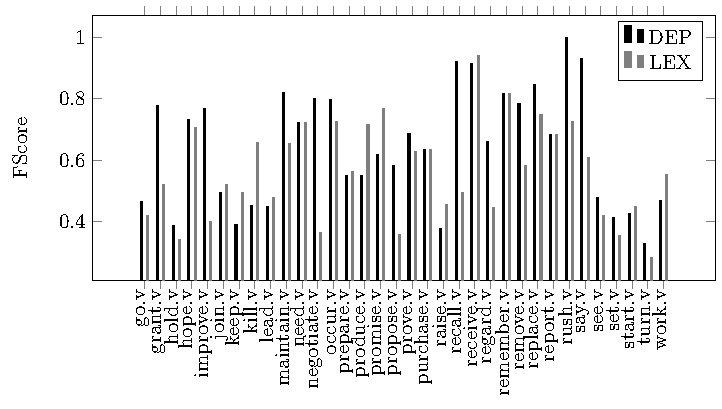
\includegraphics[width=1\linewidth]{images/Chapitre5/tex_img_files/verbs_fs_3.pdf}
\caption{Unsupervised F-Score results for the second half of verbs of the Semeval 2007 test set.}
\label{fig:verbs_fs3}
\end{figure}

%todo add phrase that says that syntactic is not as good as seen in the paper where they compare a lot of distributional models... 	


%todo split verbs?
\paragraph{Semeval-2010}
In Semeval-2010, two unsupervised evaluation metrics are introduced: \textit{V-Measure} and \textit{paired F-Score}. Briefly, the V-Measure assesses the quality of a clustering solution by measuring the degree to which each cluster consists of instances principally belonging to a single gold standard class, or homogeneity; and to completeness, the level with which each gold standard class consists of instances primarily assigned to a single cluster.

The paired F-Score evaluation transforms the clustering problem into a classification one. Two instance pairs sets are generated, the first one coming from the system induced clusters, by including pairs of the instances found in each cluster. The second set of instance pairs is built from the gold standard classes. It contains pairs of the instances found in each class. We can then define \textit{Precision} and \textit{Recall}. Precision is computed as the ratio of the number of common instance pairs between the two sets divided by the total number of pairs in the clustering solution. Recall is the count of common instance pairs between the two sets divided by the total number of pairs in the gold standard. The paired F-Score is the harmonic mean of both quantities.

Concerning the supervised evaluation, it follows explicitly that of Semeval-2007, using recall as the main performance measure as in  \cite{Semeval2010,VandeCruys2011,pedersen2010duluth}.


In Table \ref{tab:sem2010_VM} we present our systems compared to the baseline and other methods using during Semeval 2010. V-Measure is a metric well-known for favoring systems producing a higher number of clusters \cite{VandeCruys2011,pedersen2010duluth}. Thus, it is considered not a very reliable metric. We have included it to have a global insight about the performance of our method. We remark that only \textbf{LEX} performed better than both baselines, random assignation of senses (Random) and using the most frequent sense (MFS). Also, we note that we included only the best performing systems, in this case \textit{NMF$_{lib}$} and  \textit{Hermit}. The former  did not participate on the competition but was developed later. We include it henceforth to illustrate how systems variate from one position to another depending the metric used to assess the performance. The latter was the best method on this metric from the task challenge. It is important to notice that other systems exist between Hermit and \textbf{LEX}. They were not included for the sake of clarity.

The second unsupervised measure, Paired F-Score, can be seen in Table \ref{tab:sem2010_FS}. In this case both systems presented performed better than the random baseline. Any system presented was able to beat the MFS baseline. We note that \textbf{DEP} does much better compared to \textbf{LEX} concerning verbs, namely 58\% vs. 28\% F-Score. Still, the results are low considering the best results of the competition, 63\% from Duluth, although again, it generates a number of senses very similar to the MFS baseline. Both our systems induce a considerable amount of clusters while keeping a descent F-Score.

Finally, we in Table \ref{tab:sem2010_SR} we show the supervised Recall results of Semeval-2010. The best performing algorithm shown is NMF$_{lib}$. During the competition, UoY(2010) was the best method. It is a graph-based algorithm which shares the name with the UoY  system presented in Semeval-2007, but it is a different  approach. 

Concerning our systems, in this evaluation they seem to perform the best, or in a comparable level, to the top methods.  We find that in general our systems seem to perform better on the Semeval-2007 dataset. Discovering the reason could shed light into improving the performance on the Semeval-2010 test set. Given the results, it seems like a combination of features (syntactic plus lexical) in  a single algorithm could yield better results. 

As a side note, it is argued that supervised Recall is not a very robust metric as the supervised method within tends to converge towards the most frequent sense. In this regard, several researchers \cite{VandeCruys2011,pedersen2010duluth} have voiced their concerns about the quality of the current WSI/WSD evaluation metrics as well as the need of new, more robust techniques to properly evaluate these systems.

\begin{table}[]
\centering

\begin{tabular}{@{}lrrrr@{}}
\toprule
\textbf{VM (\%)} & \textbf{all} & \textbf{nouns} & \textbf{verbs} & \textbf{\#cl} \\ \midrule
{Hermit} & 16.2 & 16.7 & 15.6 & 10.78 \\
NMF$_{lib}$&11.8&13.5&9.4&4.80\\
\textbf{LEX} & 11.6 & 8.8 & 11.9 & 10.5 \\
Random & 4.4 & 4.2 & 4.6 & 4.00 \\
\textbf{DEP} & 3.5 & 3.9 & 2.8 & 2.75 \\
MFS & 0.0 & 0.0 & 0.0 & 1.00 \\ \bottomrule
\end{tabular}
\caption{Unsupervised V-Measure (VM) on the Semeval 2010 test set}
\label{tab:sem2010_VM}
\end{table}


\begin{table}[]
\centering

\begin{tabular}{@{}lrrrr@{}}
\toprule
\textbf{FS (\%)} & \textbf{all} & \textbf{nouns} & \textbf{verbs} & \textbf{\#cl} \\ \midrule
MFS & 63.5 & 57.0 & 72.4 & 1.00 \\
Duluth-WSI-SVD-Gap & 63.3 & 57.0 & 72.4 & 1.02 \\
\textbf{DEP} & 53.6 & 50.1 & 58.7 & 2.75 \\
NMF$_{lib}$&45.3&42.2&49.8&5.42\\
\textbf{LEX} & 38.4 & 46.7 & 28.5 & 10.5 \\
Random & 31.9 & 30.4 & 34.1 & 4.00 \\ \bottomrule
\end{tabular}
\caption{Unsupervised Paired F-Score (FS) for the Semeval 2010 test set}
\label{tab:sem2010_FS}
\end{table}


\begin{table}[h!]
\centering

\begin{tabular}{@{}lrrr@{}}
\toprule
\textbf{SR (\%)} & \textbf{all} & \textbf{nouns} & \textbf{verbs} \\ \midrule
NMF$_{lib}$&62.6&57.3&70.2\\
UoY(2010) & 62.4 & 59.4 & 66.8 \\

\textbf{LEX} & 59.8 & 55.8 & 67.4 \\
\textbf{DEP} & 59.3 & 53.9 & 67.2 \\
MFS & 58.7 & 53.2 & 66.6 \\
Random & 57.3 & 51.5 & 65.7 \\ \bottomrule

\end{tabular}

\caption{Supervised recall (SR) for Semeval 2010 test set (80\% mapping, 20\% evaluation)}
\label{tab:sem2010_SR}
\end{table}


\subsection{Conclusion}
We proposed a WSI/WSD method based on the contexts from the hypergraph model presented in the previous chapter. We show how using the inner links within the hypergraph structure we can group words that represent senses and then assign them to target words. Our method distinguishes from similar works in two main aspects: the definition of similarity used, the reduced number of parameters that are needed, the use of diverse types of contexts to solve the task. 	We show that our method beats said similar approaches. Also, we discovered the behavior of syntactic contexts in comparison to lexical contexts at word-level. Indeed, lexical contexts seem to perform better. This is in line with other works on distributional representations \cite{kiela2014systematic}.


\section{Combining Heterogeneous Features}
\label{chap:fusion}

%\minitoc

\subsection{Introduction}
Named Entity Recognition (NER) and Word Sense Induction and Disambiguation (WSI/ \allowbreak WSD) requires textual features to represent the similarities between words to discern between different words' meanings. NER goal is to automatically discover, within a text, mentions that belong to a well-defined semantic category. The classic task of NER involves detecting entities of type Location, Organization, Person and Miscellaneous. The task is of great importance for more complex NLP systems, e.g, relation extraction, opinion mining. Two common solutions to NER are one of the following: via matching patterns created manually or extracted semi-automatically; or by training a supervised machine learning algorithm with large quantities of annotated text. The latter being the currently more popular solution to this task.




%In the classic case of NER, we need to determine, given its context, whether a word is referring a person, a location, an organization or another miscellaneous entity. On the other hand, in WSI/WSD the goal is to determine and assign the specific meaning of a target word, again based on its context.

%Word Sense Induction and Disambiguation entails two closely related tasks\footnote{Even though these tasks are closely related, they are independent from one another. Still, in this chapter we consider them to be a single one.}. WSI aims to automatically discover the set of possible senses for a target word given a text corpus containing several occurrences of said target word. Meanwhile, WSD takes a set of possible senses and determines the most appropriate sense for each instance of the target word according to the instance's context. WSI is usually approached as an unsupervised learning task, i.e., a cluster method is applied to the words occurring in the instances of a target word. The groups found are interpreted as the senses of the target word. The WSD task is usually solved with knowledge-based approaches, based on WordNet; or more recently with supervised models which require annotated data.

As stated before, both tasks rely on features extracted from text. Usually, these representations are obtained from the surrounding context of the words in the  input corpus. Mainly,  two types of representations are used. According to their nature we call these features lexical and syntactical. 	The first type requires no extra information than that contained already in the analyzed text itself. It consists merely on the tokens surrounding a word, i.e., those tokens that come before and after within a fixed window. The second type, syntactical features, is similar to the lexical representation in that we also consider as features the tokens that appear next to the corpus' words. Nonetheless, it requires a deeper degree of language understanding. In particular, these features are based on part of speech tags, phrase constituents information, and syntactical functionality between words, portrayed by syntactical dependencies. Likewise, specific features, particular to one task are also be employed.

%For example, in NER, some standard features used in the literature include whether a word begins with an upper-case letter, the type of prefix and suffix of the word itself as well as the context words, and so on.

%In the latter case, as with any supervised model, we need to first define a set of features that will better represent each token. In this work, we make use of three different types of linguistic data, that is, (1) lexical co-occurrence, (2) grammatical dependency relations and (3) constituent-tree branch membership to try and solve the NER task. More importantly, we propose a fusion framework that uses different methods to combine these three sources of information (among others) into a single representation model.

Most of the approaches in the literature dealing with these tasks use each of these features independently or stacked together, i.e., different feature columns in an input representation space matrix. In the latter case, features are combined without regards to their nature. 

The main intuition of the present work is that word similarities may be found at different levels according to the type of features employed. In order to exploit these similarities, we look into multimedia fusion methods.  In order to better perform an analysis task, these techniques combine multimodal representations, their corresponding similarities, or the decisions coming from models fitted with these features. In our experiments, we try to mutually complement independent representations by utilizing said fusion techniques to combine (or fuse) features in the hope of improving the performance of the tasks at hand, specially compared to the use of features independently. 

Fusion techniques have previously shown their efficiency, mainly on image-related tasks, where there is a need to model the relation  between images and text extracts.
%
%. 
%
Here, in order to apply multimedia fusion techniques, we consider that the textual features  come from different modalities. The main contribution of this work is to assess the effectiveness of simple yet untested techniques to combine classical and easy to obtain textual features. As a second contribution, we propose a series of feature combination and recombination to attain better results. 

The rest of the chapter is organized as follows: in section \ref{chap6:back}, we go into further details about fusion techniques. 
%as well as its application in the NLP domain. 
We introduce the fusion operators that we use in our experiments in section \ref{chap6:application}. Then, in section \ref{chap6:expes} we show the effectiveness of the presented methods by testing them on NER and WSI/WSD and their respective datasets. Finally, in section \ref{chap6:conclusion} we present our conclusions and future directions to explore. A more general overview on fusion for multimedia analysis can be found in \cite{AtreyHEK10}.

%\subsection{Background and Related Work}
%\label{chap6:back}
% 
%We first describe below the fusion techniques we use in our methodology as well as relevant use cases where they have been employed. Then, we focus exclusively on fusion techniques applied to NLP tasks, which is the general domain of the two tasks (NER and WSI/WSD) we focus on.                                                                                                                 
%\paragraph{Multimodal Fusion Techniques}
%Multimodal fusion is a set of popular techniques used in multimedia analysis tasks. T\textit{}hese methods integrate multiple media features, the affinities among these attributes or the decisions obtained from systems trained with said features, to obtain rich insights about the data being used and thus to solve a given analysis  task \cite{AtreyHEK10}. We note that these techniques come at the price of augmenting the complexity of a given system by increasing or reducing the sparsity of a given feature matrix.
%
%
%In the multimodal fusion literature we can discern two main common types of techniques: early fusion and late fusion. 
%\paragraph{Early Fusion}
%This technique is the most widely used fusion method. The principle is simple: we take both modal features and concatenate them into a single representation matrix. More formally, we consider two matrices  that represent different modality features each  over the same set of individuals. To perform early fusion we concatenate them column-wise, such that we form a new matrix having the same number of lines but increasing the number of columns to the sum of the number of columns of both matrices. The matrices may also be weighted as to control the influence of each modality.
%
%The main advantage of early fusion is that a single unique model is fitted while leveraging the correlations among the concatenated features. The method is also easy to integrate into an analysis system. The main drawback is that we increase the representation space and may make it harder to fit models over it.
%%
%
%%   of shape $(n, m + p)$. Following the literature notation of [vulic], the early fusion representation matrix EF is defined as:
%%\begin{equation}
%%EF = \alpha \times X_1 || (1 - \alpha) \times X_2
%%\end{equation}
%
%%where $||$ represents the column-wise concatenation operation and ? is the parameter that determines the contribution of each modality. 
%%
%%Early fusion has been employed in several multimodal tasks. For example, [?]. 
%\paragraph{Late Fusion}
%In contrast to early fusion, in late fusion the combination of multimodal features are generally performed at the decision level, i.e., using the output of independent models trained  each with an unique set of features \cite{ClinchantAC11}. In this setting,  decisions produced by each model are combined into a single final result set.
%%
%The methods used to combine preliminary decisions usually involve one of two types: rule-based (where modalities are combined according to domain-specific knowledge) or linear fusion (e.g., weighting and then adding or multiplying both matrices together). This type of fusion is very close to the so-called ensemble methods in the machine learning literature.
%%
%Late fusion combines both modalities in the same semantic space. In that sense,  we may also combine modalities via an affinity representation instead of final decision sets. In other words, we can combine two modality matrices by means of their respective similarities. A final representation is then usually obtained by adding the weighted similarity matrices.
%%
%
%The advantages of late fusion include the combination of features at the same level of representation (either the fusion of decisions or similarity matrices). Also, given that independent models are trained separately, we can chose which algorithm is more adequate for each type of
%features.
%
%%For example, in information retrieval (Ah-Pine et al., 2015), lexicon learning (Vulic et al., 2016), coreference resolution (Eisenstein and Davis, 2007); different types of representations (different modalities) can be combined in order to take advantage of the complementarity existing among them
%\paragraph{Cross-media Similarity Fusion}
%%
%A third type of fusion technique, cross-media similarity fusion (or simply cross fusion),   introduced in \cite{Ah-PineCC15,ClinchantAC11}, is defined and employed to propagate a single similarity matrix into a second similarity matrix. In their paper, the authors propagated information from textual media towards visual media. In our case, we transfer information among textual features. For example, to perform a cross fusion between lexical and syntactical features, we perform the following steps: 
%\begin{enumerate}
%\item Compute the corresponding similarity matrices for each type of feature.
%\item Select only the $k$-nearest neighbor for each word within the lexical similarity matrix. These neighbors are to be used as lexical representatives to enrich the syntactical similarities.
%\item Linearly combine both similarity matrices (lexical $k$-nearest lexical neighbors with the syntactical features) via a matrix product.
%\end{enumerate}  
%
%Cross fusion aims to bridge the semantic gap between two modalities by using the most similar neighbors as proxies to transfer valuable information  from one modality onto another one. Usually, the result of a cross fusion is combined with the previous techniques, early and late fusion. In this work we perform  experiment in that sense.
%
%\paragraph{Hybrid Fusion}
%We may leverage the advantages of the previous two types of fusion techniques by combining them once more in a hybrid setting. As described in \cite{AtreyHEK10,yu2014informedia}, the main idea is to simultaneously combine features at the feature level, i.e., early fusion, and at the same semantic space or decision level. Nonetheless, they define a specific type of hybrid fusion. In this chapter, we adopt a looser definition of hybrid fusion. That is, we perform hybrid fusion by leveraging the combination of the fusion strategies described before.

We consider the first three types of fusion techniques described in the Chapter \ref{sec:fusion} (early fusion, late fusion and cross fusion) as the building blocks to the experiments we conduct.  While we work with a single modality, i.e., textual data, we consider the different kinds of features extracted from it as distinct modalities. Our intuition being that the semantic similarities among words in these different spaces can be combined in order to exploit the latent complementarity between the lexical and syntactical representations. The fusion should therefore improve the performance of the NLP tasks at hand, NER and WSI/WSD.

Our first goal is to assess the effectiveness of the classic fusion methods and then, as a second goal, to propose new combinations that yield better outcomes in terms of performance than the simpler approaches. The new combinations are found empirically. Nonetheless, as we will show, their effectiveness replicates to different datasets and NLP tasks. As will be clear in the next sections, the ways in which we tackle the tasks are, by themselves, mostly not original. We focus specially on the generation of new representation spaces. We use well-proven methods to solve both WSI/WSD and NER, so that comparisons with other systems may make more sense.
%In a general sense,
%having two similarity matrices $S_1$ and $S_2$ defined as above, we define the cross-media similarity fusion as:
%
%\begin{equation}
%XF = \mathbf{K}(S_1, k) \cdot S_2
%\end{equation}
%
%where $\mathbf{K}$ is a row-wise function that keeps only the top-k values of the similarity matrix S 1 and
%assigns zero to the rest of the line.

%In Table [] we show a synthetic table with the literature works on fusion cited in this section. We present the task solved by each contribution, the type of fusion used, the modalities involved and finally the performance gain obtained while using the fusion techniques.

%\subsection{NER and WSI/WSD}
%Previously we introduced NLP works that made use of a fusion strategy to improve a single modality system. Nonetheless, and to the best of our knowledge, there is no work that addresses NER directly while using fusion techniques from the multimedia analysis domain.

\subsection{Proposed Method}
\label{chap6:application}
 Our first goal is to assess the effectiveness of the classic fusion methods and then, as a second goal, to propose new combinations that yield better outcomes in terms of performance than the simpler approaches. The new combinations are found empirically. Nonetheless, as we will show, their effectiveness replicates to different datasets and NLP tasks. 

In the present subsection we address the core of the work performed in this chapter.
We formally describe the fusion techniques we employ in the next section. Also, we  delineate the procedure followed in our experiments. 


%This kind of fusion combinations is somewhat similar to previously employed approaches which join early fusion with cross fusion operators to construct random-walk based fusion methods \cite{Ah-PineCC15,GialampoukidisM16}. These techniques iterate over the fusion operators several times in the hopes of better propagating useful information across modalities. Still, we do not perform any kind of iteration. Our approaches perform a single step to obtain a representation matrix.



\begin{figure*}[t]
\centering
\caption{Steps followed on our experiments. First the corpus is preprocessed, then features are extracted from the text. A fusion matrix is generated, which in turn is used as input to a learning algorithm. Finally, the system yields its results and to be analyzed.}
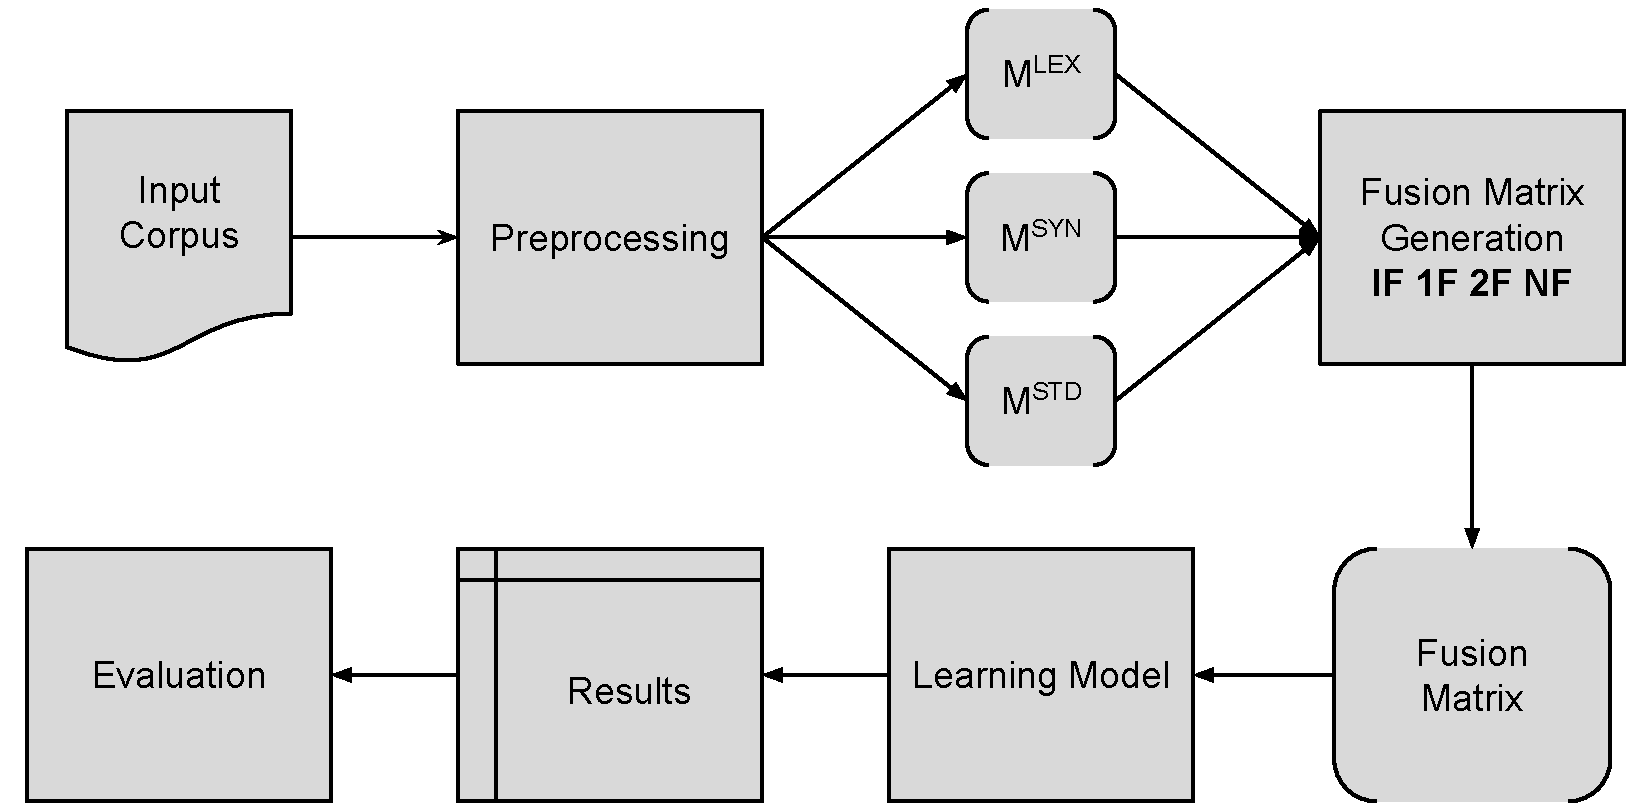
\includegraphics[width=0.85\linewidth]{images/Chapitre6/diag_metodo.pdf}

\label{fig:diagmetodo}
\end{figure*}

The experiments we carry on consist in generating fusion matrices that will serve as input to a learning algorithm in order to solve NER and WSI/WSD. These input feature matrices are based upon lexical, syntactical, or other types of representation. The procedure can be sen in Figure \ref{fig:diagmetodo}.

\subsubsection{Fusion Strategies}
We begin by presenting a  formal definition of the fusion techniques employed and described in the previous sections. We define (weighted) early fusion, late fusion and cross fusion as follows:
\paragraph{Early Fusion}
\begin{equation}
E(A,B) = \mathbf{hstack}(A , B)
\end{equation}
\paragraph{Weighted Early Fusion}
\begin{equation}
wE_\alpha(A,B) = \mathbf{hstack}(\alpha\cdot A , (1-\alpha)\cdot B)
\end{equation}
\paragraph{Late Fusion}
\begin{equation} \label{eq:late-fusion}
L_\beta(A,B) = \beta \cdot A + (1 - \beta)\cdot B
\end{equation}
\paragraph{Cross fusion}
\begin{equation}
X_{\gamma}(A,B) = \mathbf{K}(A,\gamma) \times B
\end{equation}

%\vspace{.3cm}

Parameters $A$ and $B$ are arbitrary input matrices. They may initially represent, for example,  the lexical ($M^{LEX}$) or syntactical based ($M^{SYN}$) features matrix, or their  corresponding similarity matrices, $S^{LEX}$ and  $S^{SYN}$, ~respectively. In a broader sense, matrices $A$ and $B$ may represent any pair of valid\footnote{Valid in terms of having compatible shapes while computing a matrix sum or multiplication.} fusion matrices. 

In early fusion, $E(A,B)$, the matrices $A$ and $B$ are combined together via a concatenation function $\mathbf{hstack}$ which joins both of them column-wise. Weighted early fusion  represents the same operation as before with an extra parameter: $\alpha$, which controls the relative importance of each matrix. In the following, we refer to both operations as early fusion. When $\alpha$ is determined, we refer to weighted early fusion.

Regarding late fusion $L_\beta(A,B)$, the  $\beta$ parameter determines again the importance of the  matrix $A$,  and consequently also the relevance of matrix $B$.

In cross fusion $X_\gamma(A,B)$, the $\mathbf{K}(\cdot)$ function keeps the top-$\gamma$ closest words (columns) to each word (lines) while the rest of the values are set to zero. 

Using the previously defined operators, we distinguish four levels of experiments: 
\begin{enumerate}
\item \textbf{Single Features}: in this phase we consider the modalities independently as input to the learning methods. For instance, we may train a model for NER using only the lexical features matrix $M^{LEX}$.
\item \textbf{First Degree Fusion}: we  consider the  three elementary fusion techniques by themselves (early fusion, late fusion, cross fusion) without any recombination.  These experiments, as well as those from the previous level, serve as the baselines we set to surpass in order to show the efficacy of the rest of the fusion approaches.
As an example, we may obtain a representation matrix by performing an early fusion between the lexical matrix and the syntactical features matrix: $E(M^{LEX}, M^{SYN})$. In this level we distinguish two types of cross fusion: Cross Early Fusion (XEF) and Cross Late Fusion (XLF). The first one combines a similarity matrix with a feature matrix: $X(\slex, \msyn)$. The second one joins a similarity matrix with a similarity matrix: $X(\ssyn, \slex)$.
\item \textbf{Second Degree Fusion}:  we recombine the outputs of the previous two levels with the elementary techniques. This procedure then yields a recombination of "second-degree" among fusion methods. We introduce the four types of second degree fusions in the following list. Each one is illustrated with an example:

\begin{enumerate}
\item Cross Late Early Fusion (XLEF): $X(X(\sstd, \ssyn), \mstd)$
\item Cross Early Early Fusion (XEEF: $X(\sstd, X(\sstd, \ssyn))$
\item Early Cross Early Fusion (EXEF): $E(\mstd,X(\slex, \mstd))$
\item Late Cross Early Fusion (LXEF): $L(\mstd, X(\sstd, \mstd))$
\end{enumerate}

% A second-degree fusion would be an early fusion of the lexical feature matrix with a cross fusion, expressed as $E(M^{LEX}, \allowbreak X(S^{STD}, M^{STD}))$.   
\item \textbf{N-Degree Fusion}: in this last level we follow a similar approach to the previous level by combining the output of the second-degree fusion level multiple times (more than two times, or $N>2u$) with other second-degree fusion outputs. 
Again, in this level we test the following two fusion operations:
\begin{enumerate}
\item Early Late Cross Early Fusion (ELXEF): $E(\mstd, \allowbreak L(\mstd, X(\sstd, \mstd)))$
\item Early ELXEF (EELXEF): $E(\mlex, E(E(\mstd,  L(\mstd, X(\sstd, \mstd))),\allowbreak L(\mlex, X(\ssyn, \mlex))))$
\end{enumerate}

%As an example, the equation $E(L(M^{STD}, \allowbreak X(S^{STD}, M^{STD})),  L(M^{LEX}, X(S^{SYN}, M^{LEX})))$  \allowbreak denotes the early fusion between two operations: (1) a late fusion between a lexical-features matrix and a cross fusion, and (2),  another late fusion consisting of a standard-features matrix (this matrix is detailed below)  and a cross fusion. In general, we determine a n-degree fusion empirically. That is to say, we look at the performance of second-degree fusions and try to improve the performance of the systems by recombining the fusion outputs via a n-degree combination. This process is in fact applied during the second-degree fusions also. 
	\end{enumerate}   
\subsubsection{Feature Matrices}
In the previous subsection we presented the fusion operators used in our experiments. Below we detail the three types of features used to describe the words of the corpus tested.
\paragraph{Lexical Matrix (LEX)}
For each token in the corpus, we use a lexical window of two words to the left and two words to the right, plus the token itself. Specifically, for a target word $w$, its lexical context is $(w_{-2}, w_{-2}, w, w_{+1}, w_{+2})$. This type of context features is typical for most systems studying the surroundings of a word, i.e., using a distributional approach \cite{LevyG14}.
% We retake the example phrase from \cite{LevyG14}, the lexical-based features of the phrase \textit{Australian scientist discovers start with telescope}, are shown in Table \ref{tab:lex-contexts}.
%\begin{table*}[ht]
%\centering
%\begin{tabular}{ll}
%\hline 
% \textbf{Word} & \textbf{Features} \\ 
%\hline 
%Australian & word:Australian, word+1:scientist, word+2:discovers\\ 
%scientist  &  word-1:Australian, word:scientist, word+1:discovers, word+2:star\\ 
%discovers & word-2:Australian, word-1:scientist, $\dots$, word+2:telescope \\ 
%star & word-2:scientist, word-1:discovers, word:star, $\dots$, word+2:telescope \\ 
%with & word-2:discovers, word-1:star, word:with, word+1:telescope \\ 
%telescope  &  word-2:star, word-1:with, word:telescope \\ 
%\hline \
%\end{tabular} 
%\label{tab:lex-contexts}
%\caption{Lexical features corresponding to the phrase \textit{Australian scientist discovers start with telescope}.}
%\end{table*} 

\paragraph{Syntactical Matrix (SYN)}
Based on the syntactic features used in   \cite{LevyG14,Panchenko2017}, we derive contexts based on the syntactic relations a word participates in, as well as including the part of speech (PoS) of the arguments of these relations. Formally, for a word $w$ with modifiers $m_1, \dots, m_k$ and their corresponding PoS tags $p^m_1, \dots, p^m_k$; a head $h$ and its corresponding PoS tag $p_h$, we consider the context features $(m_1, p_{m_1}, lbl_1), \dots, \allowbreak (m_k, p_{m_k}, lbl_k), \allowbreak (h,p_h,lbl\_inv_h)$. In this case, $lbl$ and $lbl_{inv}$ indicate the label of the dependency relation and its inverse, correspondingly. Using syntactic dependencies as features should yield more specific similarities, closer to synonymy, instead of the broader topical similarity found through lexical contexts.
%For the phrase \textit{Australian scientist discovers start with telescope} the dependency-based context is shown in Table \ref{tab:syn-contexts}.
\paragraph{NER Standard Features Matrix (STD)}
The features used for NER are based roughly on the same as those used in \cite{Daume2006,Balasuriya2009}. The feature set consists of: the word itself, whether the word begins with capital letter, prefix and suffix up to three characters (within a window of two words to the left and two words to the right), and the PoS tag of the current word. These features are considered to be standard in the literature. We note that the matrix generated with these features is exclusively used in the experiments regarding NER.	

\subsubsection{Learning Methods}
We use supervised and unsupervised learning methods for NER and WSI/WSD respectively. On the one hand, for NER, as supervised algorithm, we use an averaged structured perceptron \cite{Collins2002,Daume2006} to determine the tags of the named entities. We considered Logistic Regression and linear SVM. We chose the perceptron because of its performance and the lower training time.

On the other hand, for WSI/WSD, specifically for the induction part, we applied spectral clustering, as in  \cite{GoyalH14}, on the input matrices in order to automatically discover senses (a cluster is considered a sense). Regarding disambiguation, we trivially assign senses to the target word instances according to the number of common words in each cluster and the context words of the target word. In other words, for each test instance of a target word, we select the cluster (sense) with the maximum number of shared words with the current instance context.


%\begin{table*}
%\centering
%\begin{tabular}{ll}
%\hline 
% Word & Contexts \\ 
%\hline 
%Australian & scientist/NN/amod\_inv \\ 
%scientist  &  Australian/JJ/amod, discovers/VBZ/nsubj\_inv\\ 
%discovers & scientist/NN/nsubj, star/NN/dobj, telescope/NN/nmod:with \\ 
%star & discovers/VBZ/dobj\_inv \\ 
%telescope  &  discovers/VBZ/nmod:with\_inv \\ 
%\hline \
%\end{tabular} 
%\label{tab:syn-contexts}
%\caption{Syntactic contexts corresponding to the phrase \textit{Australian scientist discovers start with telescope}.}
%\end{table*}




\subsection{Experiments and Evaluation}
\label{chap6:expes}

We experiment with four levels of fusion: Single Features (SF), First-degree Fusion (1F), Second-degree Fusion (2F) and N-degree Fusion (NF). The representation matrices for NER come from lexical context features $M^{LEX}$, syntactical context features $M^{SYN}$ or standard features $M^{STD}$.  On the other hand, experiments on WSI/WSD exclusively employ matrices $M^{LEX}$ and $M^{SYN}$.

Our first goal is to compare the efficiency of the basic multimedia fusion techniques applied to  single-modality multi-feature NLP tasks, namely NER and WSI/WSD. A second goal is to empirically determine a fusion combination setting able to leverage the complementarity of our features.

To this end, we evaluate the aforementioned 4 fusion levels. We note that the fusion combinations in the third and fourth level (2F and NF) are proposed based on the results obtained in the previous levels. In other words, in order to reduce the number of experiments, we restrict our tests to the best performing configurations. This is due to the large number of possible combinations (an argument to a fusion operation may be any valid output of a second fusion operation).


\subsubsection{Named Entity Recognition}

\paragraph{Pre-processing}

As is usual when preprocessing text before performing named entity recognition, \cite{RatinovR09}, we normalize tokens that include numbers. For example, the token 1980 becomes *DDDD* and 212-325-4751 becomes *DDD*-*DDD*-*DDDD* . This allows a degree of abstraction to tokens that contain years, phone numbers, etc. We do not normalize punctuation marks.

\paragraph{Features}
The linguistic information we use are extracted with the Stanford's CoreNLP parser \cite{manning2014}. Again, the features used for these experiments on NER are those described before: lexical, syntactic and standard features, i.e., $M^{LEX}$, $M^{SYN}$, and $M^{STD}$, respectively. 

\paragraph{Test Datasets}We work with three corpus coming from different domains:
\begin{itemize}
\item [(1)] CoNLL-2003 (CONLL): This dataset was used in the language-independent named entity recognition CoNLL-2003 shared task \cite{SangM03}. It contains selected news-wire articles from the Reuters Corpus. Each article is annotated manually. It is divided in three parts:  training (\textit{train}) and two testing sets (\textit{testa} and \textit{testb}). The training part contains 219,554 lines, while the test sets contain 55,044 and 50,350 lines, respectively. The task was evaluated on the \textit{testb} file, as in the original task.
\item [(2)]WikiNER (WNER): A more recent dataset \cite{Balasuriya2009} of selected English \allowbreak Wikipedia articles, all of them annotated automatically with the author's semi-supervised \allowbreak method. In total, it contains 3,656,439 words. 
\item[(3)] Wikigold (WGLD): Also a corpus of Wikipedia articles, from the same authors of the previous corpus. Nonetheless, this was annotated manually. This dataset is the smaller, with 41,011 words. We used this corpus to validate human-tagged Wikipedia text. These three datasets are tagged with the same four types of entities: Location, Organization, Person and Miscellaneous.

%Otherwise, while it is faster to train models with this corpus, it may be the case that they are not able to properly fit the data given its size, and thus performance is lower than the other datasets.

\end{itemize}
%
\paragraph{Evaluation Measures}
We evaluate our NER models following the standard CoNLL-2003 evaluation script. Given the amount of experiments we carried on, and the size constraints, we report exclusively the total F-measure for the four types of entities (Location, Organization, Person, Miscellaneous). WNER and WGLD datasets are evaluated on a 5-fold cross validation.

\paragraph{Results}
We present in this subsection the results obtained in the named entity recognition task, while employing the 4 levels of fusion proposed in the previous section.

In contrast to other related fusion works \cite{Ah-PineCC15,ClinchantAC11,GialampoukidisM16}, we do not focus our analysis on the impact of the parameters of the fusion operators. Instead, we focus our analysis on the effect of the type of linguistic data being used and how, by transferring information from one feature type to another, they can be experimentally recombined to generate more complete representations.

Regarding the fusion operators' parameters, we empirically found the best configuration for $\beta$, from late fusion $L_\beta(A,B) = \beta \cdot A + (1 - \beta)\cdot B$, is $\beta=0.5$. This implies that an equal combination is the best linear fusion for two different types of features.

In respect of the $\gamma$ parameter, used in cross fusion $X_{\gamma}(A,B) = \mathbf{K}(A,\gamma) \times B$, we set $\gamma=5$. This indicates that just few high quality similarities attain better results than utilizing a larger quantity of lower quality similarities.

\begin{table}[!tbp]
\centering
\caption{NER F-measure results using the Single Features over the three datasets. These values serve as a first set of baselines. }
\label{tab:ner-blines}
\begin{tabular}{@{}lccc@{}}
\toprule
$A$                           & \multicolumn{3}{c}{\textbf{Single Features}} \\ \midrule
                & \textbf{CONLL}    & \textbf{WNER}     & \textbf{WGLD}    \\ \cmidrule{2-4}
$M^{\scriptscriptstyle STD}$                        & 77.41    & 77.50    & 59.66   \\
$M^{\scriptscriptstyle LEX}$                       & 69.40    & 69.17    & 52.34   \\
$M^{\scriptscriptstyle SYN}$                        & 32.95    & 28.47    & 25.49   \\ \bottomrule
\end{tabular}

\end{table}
\paragraph{Single Features}
Looking at Table \ref{tab:ner-blines}, we see that the best independent features, in terms of F-measure come from the standard representation matrix $\mstd$. This is not surprising as these features, simple as they may be, have been used and proved extensively in the NER community. On the other hand, $\mlex$ performs relatively well, considering it only includes information contained in the dataset itself. Nevertheless, this representation that this kind of lexical context features are the foundation of most word embedding techniques used nowadays.
While we expected better results from the syntactical features $\msyn$, as they are able to provide not only general word similarity, but also functional, getting close to synonymy-level \cite{LevyG14},  we believe that the relatively small size of the datasets do not provide enough information to generalize 
\paragraph{First Degree Fusion }
In Table \ref{tab:ner-1d} we present the First Degree fusion level. The best performance is obtained by trivially concatenating the representation matrices. This baseline proved to be the toughest result to beat. Late fusion does not perform well in this setting, still, we see further on that by linearly combining weighted representation matrices, we can add information to an already strong representation. Finally, regarding the cross fusion techniques, cross early and late fusion, we see that they depend directly on the information contained in the similarity matrices. We note that, as is the case on single features, the combinations with matrix $\sstd$ yield almost always the best results. While these fusion techniques by themselves may not offer the best results, we see below that by recombining them with other types of fusion we can improve the general performance of a representation.




\begin{table}[!tb]
\centering
\setlength\tabcolsep{2pt}

\caption{NER F-measure results using first degree fusion (1F). $B$ is either indicated on the table or specified as follows. Looking at EF,  $\hat{b}_{EF} = E(\msyn, \mstd)$. In XEF, ${b}^*_{\scriptscriptstyle XEF}$ takes the matrix from the set $\{M^{\scriptscriptstyle LEX}, M^{\scriptscriptstyle STD} \}$ which yields the best performing result. In XLF, $\hat{b}_{\scriptscriptstyle XLF}^{*}$ corresponds to the best performing matrix in $\{S^{\scriptscriptstyle LEX},S^{\scriptscriptstyle SYN}\}$. These configurations serve as the main set of baseline results.}
\label{tab:ner-1d}
\centering
%\tablewidth=\textwidth
\begin{tabular}{@{}llccc@{}}
\toprule
    $A$      &    $B$       & \multicolumn{3}{r}{\textbf{Early Fusion} }                                            \\ \midrule
          &           & \textbf{CONLL}                      & \textbf{WNER}                      & \textbf{WGLD}                      \\ \cmidrule{3-5}
$M^{\scriptscriptstyle LEX}$ & $M^{\scriptscriptstyle SYN}$ & 72.01                      & 70.59                     & 59.38                     \\
$M^{\scriptscriptstyle LEX}$ & $M^{\scriptscriptstyle STD}$ & 78.13                      & 79.78                     & 61.96                     \\
$M^{\scriptscriptstyle SYN}$ & $M^{\scriptscriptstyle STD}$ & 77.70                      & 78.10                     & 60.93                     \\
$M^{\scriptscriptstyle LEX}$ & $\hat{b}_{EF}$ & \textbf{78.90}                      & \textbf{80.04}                     & \textbf{63.20}                   \\
\midrule
          &           & \multicolumn{3}{r}{\textbf{Late Fusion} }                                             \\
\midrule     
          &           & \textbf{CONLL}                      & \textbf{WNER}                      & \textbf{WGLD}                      \\ \cmidrule{3-5}
$S^{\scriptscriptstyle LEX}$ & $S^{\scriptscriptstyle SYN}$ & \textbf{61.65}                      & 58.79                     & 44.29                     \\
$S^{\scriptscriptstyle LEX}$ & $S^{\scriptscriptstyle STD}$ & 55.64                      & \textbf{67.70}                     & 48.00                     \\
$S^{\scriptscriptstyle SYN}$ & $S^{\scriptscriptstyle STD}$ & 50.21                      & 58.41                     & \textbf{49.81}                     \\
\midrule
          &           & \multicolumn{3}{r}{\textbf{Cross Early Fusion}} \\
\midrule
          &           & \textbf{CONLL}                      & \textbf{WNER}                      & \textbf{WGLD}                      \\ \cmidrule{3-5}
$S^{\scriptscriptstyle LEX}$ &$M^{\scriptscriptstyle STD}$        & 49.90                      & \textbf{70.27}                     & \textbf{62.69}                    \\
$S^{\scriptscriptstyle SYN}$ & $M^{\scriptscriptstyle STD}$ & 47.27                      & 51.38                     & 48.53                     \\
$S^{\scriptscriptstyle STD}$ & ${b}^*_{\scriptscriptstyle XEF}$        & \textbf{52.89}                      & 62.21                     & 50.15                     \\
\midrule
          &           & \multicolumn{3}{r}{\textbf{Cross Late Fusion}}  \\
\midrule
          &           & \textbf{CONLL}                      & \textbf{WNER}                      & \textbf{WGLD}                      \\ \cmidrule{3-5}
$S^{\scriptscriptstyle LEX}$ & $S^{\scriptscriptstyle STD}$ & 27.75                      & \textbf{59.12}                     & 38.35                     \\
$S^{\scriptscriptstyle SYN}$ & ${b}_{\scriptscriptstyle XLF}^{*}$       & 36.87                      & 40.92                     & 39.62                     \\
$S^{\scriptscriptstyle STD}$ & ${b}_{\scriptscriptstyle XLF}^{*}$        & \textbf{41.89}                      & 52.03                     & \textbf{39.92}                     \\ \bottomrule
\end{tabular}
\end{table}


\begin{table}[t]
\centering

\caption{NER F-measure results using second degree fusion (2F). In XLEF, ${a^*}$ corresponds to the best performing matrix in the set $\{ X(S^{\scriptscriptstyle STD}, S^{\scriptscriptstyle LEX}),X(S^{\scriptscriptstyle LEX}, S^{\scriptscriptstyle STD}), \allowbreak X(S^{\scriptscriptstyle STD}, S^{\scriptscriptstyle SYN})\}$. For XEEF,  $\hat{b}_{\scriptscriptstyle XEEF}=E(\mlex, \mstd)$. In EXEF, $b^*_{\scriptscriptstyle EXEF}$  takes the best performing matrix from $\{X(\ssyn, \mlex), \allowbreak X(\slex, \mlex), X(\slex, \mstd), \allowbreak X(\ssyn, \mlex), X(\ssyn, \mstd) \}$. Finally, in LXEF, $\hat{b}_{\scriptscriptstyle LXEF}$ takes the best possible matrix from $\{X(\slex, \mstd), X(\ssyn, \mstd), \allowbreak X(\ssyn, \mlex) \}$.}
\label{tab:ner_2d}
\begin{tabular}{@{}llccc@{}}
	\toprule
	$A$                      & $B$            & \multicolumn{3}{r}{\textbf{Cross Late Early Fusion}}  \\ \midrule
	                         &                & \textbf{CONLL} & \textbf{WNER}  &             \textbf{WGLD}             \\
	\cmidrule{3-5}
$\hat{a}$ & $M^{\scriptscriptstyle STD}$      & 37.69 & 59.44 &            \textbf{41.71}             \\
	$\hat{a}$                & $M^{\scriptscriptstyle LEX}$      & \textbf{38.31} & \textbf{58.73} &            41.56             \\
	$\hat{a}$                & $M^{\scriptscriptstyle SYN}$      & 29.31 & 52.06 &            34.91             \\ \midrule
	                         &                & \multicolumn{3}{r}{\textbf{Cross Early Early Fusion}} \\ \midrule
	                         &                & \textbf{CONLL} & \textbf{WNER}  &             \textbf{WGLD}             \\
	\cmidrule{3-5}
$S^{\scriptscriptstyle STD}$ & $\hat{b}_{\scriptscriptstyle XEEF}$          &   \textbf{54.34}    &    \textbf{64.20}   & 39.59 \\
	$S^{\scriptscriptstyle LEX}$                &$\hat{b}_{\scriptscriptstyle XEEF}$         &  49.71     &   71.84    &  \textbf{45.14}\\
	$S^{\scriptscriptstyle SYN}$                & $\hat{b}_{\scriptscriptstyle XEEF}$         &  47.54     &   53.77    & 43.32 \\ \midrule
	                         &                & \multicolumn{3}{r}{\textbf{Early Cross Early Fusion}} \\ \midrule
	                         &                & \textbf{CONLL} & \textbf{WNER}  &             \textbf{WGLD}             \\
	\cmidrule{3-5}
$M^{\scriptscriptstyle STD}$ & $b^*_{\scriptscriptstyle EXEF}$          & 49.58 & \textbf{77.32} &            \textbf{61.69}             \\
	$M^{\scriptscriptstyle LEX}$                & $b^*_{\scriptscriptstyle EXEF}$      & 49.79 & 66.22 &            53.54             \\
	$M^{\scriptscriptstyle SYN}$                & $b^*_{\scriptscriptstyle EXEF}$           & \textbf{51.53} & 70.94 &            53.70             \\ \midrule
	                         &                & \multicolumn{3}{r}{\textbf{Late Cross Early Fusion}}  \\ \midrule
	                         &                & \textbf{CONLL} & \textbf{WNER}  &             \textbf{WGLD}             \\
	\cmidrule{3-5}
$M^{\scriptscriptstyle STD}$ &$\hat{b}_{\scriptscriptstyle LXEF}$           &  54.82   & \textbf{75.70} &            \textbf{54.73}             \\
	$M^{\scriptscriptstyle LEX}$                & $\hat{b}_{\scriptscriptstyle LXEF}$  & \textbf{56.53} & 62.27 &            52.39             \\ \bottomrule
\end{tabular}
\end{table}
           
\paragraph{Second Degree Fusion} 
The second degree fusion techniques presented in Table \ref{tab:ner_2d} show that the recombination of cross fusion techniques gets us closer to the early fusion baseline. With the exception of cross late early fusion, the rest of the recombination schemes yield interesting results. First, in cross early fusion, the best results, for the most part, are obtained while using the $\slex$ matrix combined with the output of $E(\mlex, \mstd)$, which is still far from the baseline values. Concerning, EXEF, we get already close to surpass the baselines with the $\mstd$ matrix, except for the CONLL dataset. In LXEF, even though the cross fusion $X(\ssyn, \mlex)$ is not the best performing, we found experimentally that by combining it with $\mlex$ through a late fusion, it gets  a strong complementary representation. Our intuition in this case was to complement $\mlex$ with itself but enriched with the $\ssyn$ information. In the N-degree fusion results we discover that indeed this propagation of information helps us beat the baselines we set before.
\paragraph{N-degree Fusion}
Finally, the last set of experiments are shown in Table \ref{tab:ner-nf1}. Using a recombination of fusion techniques, a so-called hybrid approach, we finally beat the baselines (single features and early fusion) for each dataset. We note that the best configuration made use of a weighted early fusion with $\alpha=0.95$. This indicates that the single feature matrix, $\mlex$ is enriched a small amount by the fusion recombination, which is enough to improve the results of said baselines. In CONLL, the early fusion (see Table \ref{tab:ner-1d}) baseline being 78.13, we reached 78.69, the lowest improvement of the three datasets. Regarding the Wikipedia corpus, in WNER, we went from 79.78 to 81.75; and in WGLD, from 61.96 to 67.29, the largest improvement of all.

In the next section we transfer the knowledge gained in this task to a new one, word sense induction and disambiguation.

\begin{table}[t]
\centering

\caption{F-measure results using N-degree fusion (NF). In ELXEF, $ \hat{b}_{\scriptscriptstyle ELXEF}=L(\mlex, X(\ssyn, \mlex))$. For EELXEF, $\hat{b}_{\scriptscriptstyle EELXEF} =  E(E(\mstd, 	 L(\mlex, X(\ssyn, \mlex))), \allowbreak L(\mlex, X(\sstd, \mlex)))$ for CONLL and $\hat{b}_{\scriptscriptstyle EELXEF} =  E(E(\mstd, 	 L(\mstd, X(\ssyn, \mstd))), L(\mlex, X(\ssyn, \mlex)))$ for WNER and WGLD. The best result is obtained in EELXEF when $\alpha=0.95$.}

\label{tab:ner-nf1}
\begin{tabular}{@{}llccc@{}}
\toprule
    $A$      &    $B$      & \multicolumn{3}{r}{\makecell{\textbf{Early Late} \\ \textbf{Cross Early Fusion}}}                                            \\ \midrule
          &      &      \textbf{CONLL}                     & \textbf{WNER}                      & \textbf{WGLD}                      \\ \cmidrule{3-5}
$M^{\scriptscriptstyle STD}$ & $ \hat{b}_{\scriptscriptstyle ELXEF}$ & 67.16                      & 79.45                     & 62.37                     \\
\midrule
          &        &   \multicolumn{3}{r}{\makecell{\textbf{Early Early} \\ \textbf{Late Cross Early Fusion}}}                                             \\
\midrule     
          &          & \textbf{CONLL}                      & \textbf{WNER}                      & \textbf{WGLD}                      \\ \cmidrule{3-5}
%&& EF & EF & EF \\        
%\cmidrule(l){3-3}\cmidrule(l){4-4}\cmidrule(l){5-5}

  
$M^{\scriptscriptstyle LEX}$ & $ \hat{b}_{\scriptscriptstyle EELXEF}$ & 65.01                      & 78.02                     & 62.34                    \\
$M^{\scriptscriptstyle LEX}_{\alpha=0.95}$ & $ \hat{b}_{\scriptscriptstyle EELXEF}$  & \textbf{79.67}                      & \textbf{81.79}                     & \textbf{67.05	}                     \\ \midrule
\multicolumn{2}{l}{EF Baseline} & 78.90                      & 80.04                     & 63.20                     \\ 
\bottomrule
\end{tabular}

% | B in $\{M^{\scriptscriptstyle LEX}, M^{\scriptscriptstyle STD}, M^{\scriptscriptstyle SYN}\}$
%| B in $\{S^{\scriptscriptstyle LEX}, S^{\scriptscriptstyle STD}, S^{\scriptscriptstyle SYN}\}$
\end{table}



\subsubsection{Word Sense Induction and Disambiguation}
Having learned the best fusion configuration from the previous task, in these experiments we set to test if the improvements achieved can be transfered into another NLP task, namely Word Sensed Induction and Disambiguation (WSI/WSD). As preprocessing, we simply remove stopwords and tokens with less than three letters.
% Please add the following required packages to your document preamble:
% \usepackage{booktabs}
\begin{table}[!ht]
\centering
\setlength\tabcolsep{3pt}
\caption{Supervised Recall and Unsupervised F-measure for the Semeval 2007 corpus. We also display the average number of clusters found by each fusion configuration.}
\label{ref:wsd-semeval}
\begin{tabular}{@{}lccc|cccc@{}}
\toprule
\textbf{Method} & \multicolumn{3}{c|}{\textbf{Recall (\%)}} & \multicolumn{3}{c}{\textbf{FM (\%)}} & \# \textbf{cl} \\ \midrule
       & all           & noun          & verb          & all          & noun         & verb         &\\ 
       \midrule
       & \multicolumn{7}{r}{\textbf{Single Features}} \\ \midrule
       $M^{LEX}$                    & 79.20 & 82.10 & 75.80 &	72.70	 & 76.90 & 67.90 & 4.13\\
 

       $M^{SYN}$                    & 79.10 & 81.60 & 76.20 &	69.30	& 69.40 & 69.20 & 4.47\\
       \midrule
       &            \multicolumn{7}{r}{\textbf{Early Fusion}}       \\ \midrule
       $E(M^{LEX}, M^{SYN})$		& 78.70 & 81.11 & 76.10 &	74.00	& 76.66 & 71.11 & 4.46\\
	  \midrule
       &            \multicolumn{7}{r}{\textbf{Cross Early Fusion}}       \\ \midrule	         
	   
	   $X(S^{LEX}, M^{LEX})$		& 79.20 & 82.30 & 75.70 &	76.20	& 79.60 & 72.50 & 3.63 \\	   
       $X(S^{LEX}, M^{SYN})$		& 78.30 & 80.90 & 75.30 &	74.60	& 75.10 & 73.90 & 3.08 \\
	   $X(S^{SYN}, M^{LEX})$		& 78.60 & 80.90 & 76.10 &	78.90	& 80.70 & 76.90	 & 1.08 \\	   
       $X(S^{SYN}, M^{SYN})$		& 78.90 & 81.40 & 76.10 &	73.70	& 77.70 & 70.00 & 2.72 \\       
 \midrule
       &            \multicolumn{7}{r}{\textbf{Cross Late Fusion}}       \\ \midrule
	   
 
	   $X(S^{SYN}, S^{LEX})$		& 78.70 & 80.90 & 76.20 &	78.90	& 80.80 & 76.80 & 1.01 \\
	   $X(S^{LEX}, S^{SYN})$		& 78.80 & 80.90	& 76.06 &	78.70	& 80.50  & 76.80 & 1.33 \\
	  
 \midrule
       &            \multicolumn{7}{r}{\textbf{Cross Late Early Fusion}}       \\ \midrule
	   
 


       $X(X(S^{LEX}, S^{SYN}), M^{LEX})$		& 78.40 & 80.40 & 76.10 &	70.00	&68.70  & 71.40& 3.11 \\	   
       $X(X(S^{LEX}, S^{SYN}), M^{SYN})$		& 78.90 & 81.80 & 75.60 &	75.20	& 77.40 & 72.80 & 3.16 \\	   
       	  \midrule
       &            \multicolumn{7}{r}{\textbf{Early Cross Early Fusion}}       \\ \midrule	         
       
       $E(M^{LEX}, X(S^{LEX}, M^{LEX}))$		& 79.20 & 82.40 & 75.70 &	76.00	& 79.50  & 72.10 & 3.57 \\	   
	   $E(M^{SYN}, X(S^{LEX}, M^{LEX}))$		& 78.30 & 80.50 & 75.80 &	75.20	&75.40  & 75.00 & 1.95 \\	   
       \midrule
       &            \multicolumn{7}{r}{\textbf{Late Cross Early Fusion}}       \\ \midrule	  
	   $L(M^{SYN}, X(S^{LEX}, M^{SYN}))$		& 78.60 & 81.10 & 75.80 &	67.80	& 71.40&63.80 & 4.22 \\	   
	   $L(M^{LEX}, X(S^{LEX}, M^{LEX}))$		& 79.50 & 82.80 & 75.70 &	76.09	&79.10 &72.70 & 3.96 \\	   
       \midrule
       &            \multicolumn{7}{r}{\textbf{Early Late Cross Early Fusion}}       \\ \midrule	  
	   $E(M^{LEX}, L(M^{SYN}, X(S^{LEX}, M^{SYN})))$		& 78.50 & 81.40 & 75.40 &	74.20	& 78.20 & 69.80& 4.26 \\	   
	   $E(M^{LEX}, L(M^{LEX}, X(S^{LEX}, M^{LEX})))$		& 79.50 & 82.70 & 75.90 &	75.80	& 78.50&72.70 & 3.99 \\
%	   \midrule
%	   &            \multicolumn{7}{c}{Early Early Late Cross Early Fusion}       \\ 
	   
	   
%	   Semeval-2007 Best Systems& 81.60 & 86.80 & 75.70 &	78.70	& 80.80&76.30 & 3.06, 1.15 \\ 	 
%	   Baseline 		& 78.70 & 80.90 & 76.20 &	78.90	& 80.70&76.80 & 1.00 \\ 	   	 	    
		   
       \bottomrule
       
       
\end{tabular}


\end{table}
\paragraph{Features}
We use the same set of features from the previous task, without the standard NER features, that is, those represented by $M^{STD}$, as they are specifically designed to tackle NER.
\paragraph{Test Dataset}
The WSI/WSD model is tested on the dataset of  the SEMEVAL-2007 WSID task \cite{Agirre2007}. The task was based on a set of 100 target words (65 verbs and 35 nouns), each  word having a set of instances, which are specific contexts where the word appear. Senses are induced from these contexts and applied to each one of the instances.


\paragraph{Evaluation Measures}
Being an unsupervised task, the evaluation metrics of WSI/WSD are debated in terms of quality \cite{CruysA11}. We consider supervised recall and unsupervised F-measure, as in the competition original paper \cite{Agirre2007}. The first one maps the output of a system to the true senses of the target words' instances and the second one measures the quality of the correspondence between the automatically found clusters and the senses. 
We consider that the number of senses found by the system is also a rather good indicator of performance: the best competition baseline assigns the most frequent sense to each target word (this baseline is called MFS), thus this baseline system would have an average of 1 sense (cluster) per word. A system that goes near this average may be indeed not resolving the task efficiently but finding the MFS trivial solution. Consequently, to show that we do not fall in the MFS solution, we display in our results the average number of clusters.

\subsection{Results and Discussion}
Word sense induction and disambiguation results are found in Table \ref{ref:wsd-semeval}. Again, we aim to surpass the baseline of the single features and early fusion.  We experimentally set $\beta=0.90$ and $\gamma=50$. In this task, in late fusion, when the first matrix  is deemed more relevant than the second one, the performance is higher. This may be due to the fact that, in this task, the feature matrices rows contain types (that is, each line represent an unique word), and thus they are more dense, which may entail more noisy data. By reducing the relevance of the second matrix in late fusion, we are effectively attenuating the less important information. Regarding $\gamma=50$, again due to the denser characteristic of the matrices, there is a larger quantity of true similar words that are useful to project information into another matrix, through cross fusion.  

The WSI/WSD results are shown in Table \ref{ref:wsd-semeval}. In the following paragraph, we will discuss these result all at once. Due to the page limit constraint, we omit certain configurations that do not yield interesting results either by converging to the MFS solution (1 sense found per target word) or because the performance shown by those  configurations is not interesting.

Regarding Single Features, $\mlex$ comes on top of $\msyn$ again. Nonetheless, $\msyn$ is much closer in terms of performance, and as expected, it is actually higher with regards to verbs. 

On the 1F level, we see that the early fusion technique in this task does not surpass the independent features representation. Our intuition is that the similarities of both matrices seem to be correlated. In cross early fusion, the best result is obtained by $X(\slex, \mlex)$,  regarding the unsupervised F-measure. This configuration already beats our baselines, improving both noun and verb results on the unsupervised evaluation, improving the supervised recall of nouns, and staying on the same level considering all words. Also, it produces more senses than the MSF average number of senses (1 sense per target word), which is good but not indicative of results correctness. Regarding cross late fusion, given the average number of clusters produced, it seems that both results converge towards the MFS, therefore we do not consider these results.

Beginning with the fusion recombinations, in level 2F, both cross late early fusions yield average results. In cross early cross early fusion, the early fusion of $\mlex$ with  $X(\slex, \mlex)$ yields very similar results than $X(\slex, \mlex)$. The next natural step is to test this fusion via a linear combination, with a late fusion. The result obtained confirmed the intuition of enriching a single feature matrix with another weighted-down matrix to improve the performance. Indeed, we consider that $L(M^{LEX}, X(S^{LEX}, M^{LEX}))$ gets the best results in terms of all-words supervised recall and the second best all-words unsupervised F-measure (we do not consider solutions that are too close to the MFS baseline). 

We test the same configurations as in NER, within the NF level, to try and improve our results. Nonetheless, in general, they do not overcome the best result found previously.
In general, we found that the recombination fusion techniques work in terms of improving the performance of the tasks addressed.

In the following, we discuss how each type of feature affects the performance of individual classes in NER or the senses discovered in WSI/WSD.

%\subsection{Feature Importance Analysis}
%\subsubsection{WSI/WSD}
%\subsubsection{NER}

\subsection{Conclusion}
\label{chap6:conclusion}
We presented  a comparative study of multimedia fusion techniques applied to two NLP tasks: Named Entity Recognition and Word Sense Induction and Disambiguation. We also proposed new fusion recombinations in order to complement the information contained in the single representation matrices. In order to accomplish this goal, we built upon basic fusion techniques such as early and late fusion, as well as cross media fusion to transfer quality information from one set of features to another. 

We found that by taking a strong feature, in our case lexical context, $\mlex$, and enriching it with the output of rather complex fusion combinations, we can improve the performance of the tasks addressed. The enrichment has to give more relevance to the strong feature matrix, by selecting the right parameters. 

While there is an improvement, we do note that fusion techniques augment the complexity of the tasks at hand by enlarging the feature space or making it more dense.

In that sense, more intelligent ways of finding the most appropriate fusion must be researched. This is indeed one of our future work paths: determining an optimal fusion path from single features to a N-degree fusion recombination. Coupled with this, the automatic determination of the parameters is still ongoing research in the multimedia fusion community. Consequently, we believe that efficiently determining both parameters and fusion combinations is the general domain of our future work. Another route we would like to explore is testing these techniques on other tasks and with datasets from different domains, in order to assert its effectiveness.

